\documentclass{standalone}
\usepackage{tikz}
\usetikzlibrary{patterns, positioning}


\begin{document}
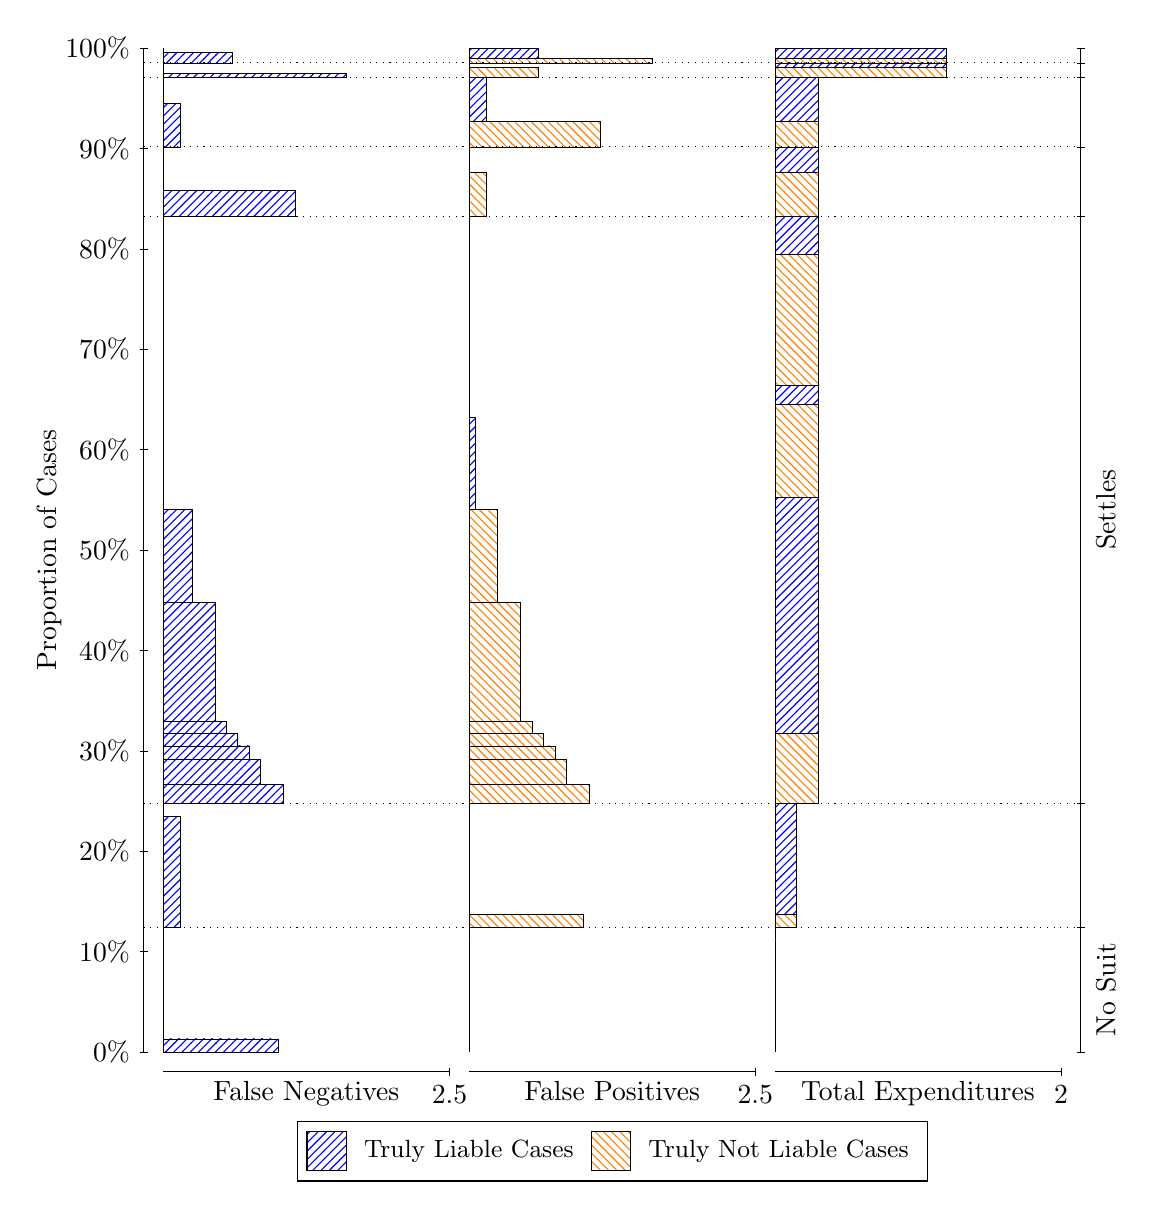
\begin{tikzpicture}
\draw[black, very thin] (1.5,1.75) -- (1.5,14.5);
\node[rotate=90, text=black, anchor=center] at (0.3, 8.125) {Proportion of Cases};
\draw[black, very thin] (1.45,1.75) -- (1.55,1.75);
\node[text=black, anchor=east] at (1.45, 1.75) {0\%};
\draw[black, very thin] (1.45,3.025) -- (1.55,3.025);
\node[text=black, anchor=east] at (1.45, 3.025) {10\%};
\draw[black, very thin] (1.45,4.3) -- (1.55,4.3);
\node[text=black, anchor=east] at (1.45, 4.3) {20\%};
\draw[black, very thin] (1.45,5.575) -- (1.55,5.575);
\node[text=black, anchor=east] at (1.45, 5.575) {30\%};
\draw[black, very thin] (1.45,6.85) -- (1.55,6.85);
\node[text=black, anchor=east] at (1.45, 6.85) {40\%};
\draw[black, very thin] (1.45,8.125) -- (1.55,8.125);
\node[text=black, anchor=east] at (1.45, 8.125) {50\%};
\draw[black, very thin] (1.45,9.4) -- (1.55,9.4);
\node[text=black, anchor=east] at (1.45, 9.4) {60\%};
\draw[black, very thin] (1.45,10.675) -- (1.55,10.675);
\node[text=black, anchor=east] at (1.45, 10.675) {70\%};
\draw[black, very thin] (1.45,11.95) -- (1.55,11.95);
\node[text=black, anchor=east] at (1.45, 11.95) {80\%};
\draw[black, very thin] (1.45,13.225) -- (1.55,13.225);
\node[text=black, anchor=east] at (1.45, 13.225) {90\%};
\draw[black, very thin] (1.45,14.5) -- (1.55,14.5);
\node[text=black, anchor=east] at (1.45, 14.5) {100\%};

\draw[black, very thin] (13.4,1.75) -- (13.4,14.5);
\draw[black, very thin] (13.35,1.75) -- (13.45,1.75);
\node[anchor=west] at (13.35, 1.75) {};
\draw[black, very thin] (13.35,3.3316) -- (13.45,3.3316);
\node[anchor=west] at (13.35, 3.3316) {};
\draw[black, very thin] (13.35,4.9074) -- (13.45,4.9074);
\node[anchor=west] at (13.35, 4.9074) {};
\draw[black, very thin] (13.35,12.366) -- (13.45,12.366);
\node[anchor=west] at (13.35, 12.366) {};
\draw[black, very thin] (13.35,13.245) -- (13.45,13.245);
\node[anchor=west] at (13.35, 13.245) {};
\draw[black, very thin] (13.35,14.123) -- (13.45,14.123);
\node[anchor=west] at (13.35, 14.123) {};
\draw[black, very thin] (13.35,14.311) -- (13.45,14.311);
\node[anchor=west] at (13.35, 14.311) {};
\draw[black, very thin] (13.35,14.5) -- (13.45,14.5);
\node[anchor=west] at (13.35, 14.5) {};

\draw[black, very thin, pattern color=blue, pattern=north east lines] (1.75,1.75) rectangle (3.2033,1.9164);
\draw[black, very thin, pattern color=orange, pattern=north west lines] (1.75,1.9164) rectangle (1.75,3.3316);
\draw[black, very thin, pattern color=blue, pattern=north east lines] (1.75,3.3316) rectangle (1.968,4.7438);
\draw[black, very thin, pattern color=orange, pattern=north west lines] (1.75,4.7438) rectangle (1.75,4.9074);
\draw[black, very thin, pattern color=blue, pattern=north east lines] (1.75,4.9074) rectangle (3.276,5.1491);
\draw[black, very thin, pattern color=blue, pattern=north east lines] (1.75,5.1491) rectangle (2.9853,5.4622);
\draw[black, very thin, pattern color=blue, pattern=north east lines] (1.75,5.4622) rectangle (2.84,5.6372);
\draw[black, very thin, pattern color=blue, pattern=north east lines] (1.75,5.6372) rectangle (2.6947,5.7981);
\draw[black, very thin, pattern color=blue, pattern=north east lines] (1.75,5.7981) rectangle (2.5493,5.9453);
\draw[black, very thin, pattern color=blue, pattern=north east lines] (1.75,5.9453) rectangle (2.404,7.4578);
\draw[black, very thin, pattern color=blue, pattern=north east lines] (1.75,7.4578) rectangle (2.1133,8.6368);
\draw[black, very thin, pattern color=orange, pattern=north west lines] (1.75,8.6368) rectangle (1.75,12.366);
\draw[black, very thin, pattern color=blue, pattern=north east lines] (1.75,12.366) rectangle (3.4213,12.693);
\draw[black, very thin, pattern color=orange, pattern=north west lines] (1.75,12.693) rectangle (1.75,13.245);
\draw[black, very thin, pattern color=blue, pattern=north east lines] (1.75,13.245) rectangle (1.968,13.796);
\draw[black, very thin, pattern color=orange, pattern=north west lines] (1.75,13.796) rectangle (1.75,14.123);
\draw[black, very thin, pattern color=blue, pattern=north east lines] (1.75,14.123) rectangle (4.0753,14.18);
\draw[black, very thin, pattern color=orange, pattern=north west lines] (1.75,14.18) rectangle (1.75,14.311);
\draw[black, very thin, pattern color=blue, pattern=north east lines] (1.75,14.311) rectangle (2.622,14.443);
\draw[black, very thin, pattern color=orange, pattern=north west lines] (1.75,14.443) rectangle (1.75,14.5);
\draw[black, very thin, pattern color=orange, pattern=north west lines] (5.6333,1.75) rectangle (5.6333,3.1652);
\draw[black, very thin, pattern color=blue, pattern=north east lines] (5.6333,3.1652) rectangle (5.6333,3.3316);
\draw[black, very thin, pattern color=orange, pattern=north west lines] (5.6333,3.3316) rectangle (7.0867,3.4951);
\draw[black, very thin, pattern color=blue, pattern=north east lines] (5.6333,3.4951) rectangle (5.6333,4.9074);
\draw[black, very thin, pattern color=orange, pattern=north west lines] (5.6333,4.9074) rectangle (7.1593,5.149);
\draw[black, very thin, pattern color=orange, pattern=north west lines] (5.6333,5.149) rectangle (6.8687,5.4622);
\draw[black, very thin, pattern color=orange, pattern=north west lines] (5.6333,5.4622) rectangle (6.7233,5.6371);
\draw[black, very thin, pattern color=orange, pattern=north west lines] (5.6333,5.6371) rectangle (6.578,5.798);
\draw[black, very thin, pattern color=orange, pattern=north west lines] (5.6333,5.798) rectangle (6.4327,5.9452);
\draw[black, very thin, pattern color=orange, pattern=north west lines] (5.6333,5.9452) rectangle (6.2873,7.4578);
\draw[black, very thin, pattern color=orange, pattern=north west lines] (5.6333,7.4578) rectangle (5.9967,8.6369);
\draw[black, very thin, pattern color=blue, pattern=north east lines] (5.6333,8.6369) rectangle (5.706,9.816);
\draw[black, very thin, pattern color=blue, pattern=north east lines] (5.6333,9.816) rectangle (5.6333,12.366);
\draw[black, very thin, pattern color=orange, pattern=north west lines] (5.6333,12.366) rectangle (5.8513,12.918);
\draw[black, very thin, pattern color=blue, pattern=north east lines] (5.6333,12.918) rectangle (5.6333,13.245);
\draw[black, very thin, pattern color=orange, pattern=north west lines] (5.6333,13.245) rectangle (7.3047,13.571);
\draw[black, very thin, pattern color=blue, pattern=north east lines] (5.6333,13.571) rectangle (5.8513,14.123);
\draw[black, very thin, pattern color=orange, pattern=north west lines] (5.6333,14.123) rectangle (6.5053,14.254);
\draw[black, very thin, pattern color=blue, pattern=north east lines] (5.6333,14.254) rectangle (5.6333,14.311);
\draw[black, very thin, pattern color=orange, pattern=north west lines] (5.6333,14.311) rectangle (7.9587,14.368);
\draw[black, very thin, pattern color=blue, pattern=north east lines] (5.6333,14.368) rectangle (6.5053,14.5);
\draw[black, very thin, pattern color=orange, pattern=north west lines] (9.5167,1.75) rectangle (9.5167,3.1652);
\draw[black, very thin, pattern color=blue, pattern=north east lines] (9.5167,3.1652) rectangle (9.5167,3.3316);
\draw[black, very thin, pattern color=orange, pattern=north west lines] (9.5167,3.3316) rectangle (9.7892,3.4951);
\draw[black, very thin, pattern color=blue, pattern=north east lines] (9.5167,3.4951) rectangle (9.7892,4.9074);
\draw[black, very thin, pattern color=orange, pattern=north west lines] (9.5167,4.9074) rectangle (10.062,5.798);
\draw[black, very thin, pattern color=blue, pattern=north east lines] (9.5167,5.798) rectangle (10.062,8.7976);
\draw[black, very thin, pattern color=orange, pattern=north west lines] (9.5167,8.7976) rectangle (10.062,9.9767);
\draw[black, very thin, pattern color=blue, pattern=north east lines] (9.5167,9.9767) rectangle (10.062,10.218);
\draw[black, very thin, pattern color=orange, pattern=north west lines] (9.5167,10.218) rectangle (10.062,11.878);
\draw[black, very thin, pattern color=blue, pattern=north east lines] (9.5167,11.878) rectangle (10.062,12.366);
\draw[black, very thin, pattern color=orange, pattern=north west lines] (9.5167,12.366) rectangle (10.062,12.918);
\draw[black, very thin, pattern color=blue, pattern=north east lines] (9.5167,12.918) rectangle (10.062,13.245);
\draw[black, very thin, pattern color=orange, pattern=north west lines] (9.5167,13.245) rectangle (10.062,13.571);
\draw[black, very thin, pattern color=blue, pattern=north east lines] (9.5167,13.571) rectangle (10.062,14.123);
\draw[black, very thin, pattern color=orange, pattern=north west lines] (9.5167,14.123) rectangle (11.697,14.254);
\draw[black, very thin, pattern color=blue, pattern=north east lines] (9.5167,14.254) rectangle (11.697,14.311);
\draw[black, very thin, pattern color=orange, pattern=north west lines] (9.5167,14.311) rectangle (11.697,14.368);
\draw[black, very thin, pattern color=blue, pattern=north east lines] (9.5167,14.368) rectangle (11.697,14.5);
\draw[black, dotted] (1.5,3.3316) -- (13.4,3.3316);
\draw[black, dotted] (1.5,4.9074) -- (13.4,4.9074);
\draw[black, dotted] (1.5,12.366) -- (13.4,12.366);
\draw[black, dotted] (1.5,13.245) -- (13.4,13.245);
\draw[black, dotted] (1.5,14.123) -- (13.4,14.123);
\draw[black, dotted] (1.5,14.311) -- (13.4,14.311);
\draw[black, very thin] (1.75,1.5) -- (5.3833,1.5);
\node[text=black, anchor=north] at (3.5667, 1.5) {False Negatives};
\draw[black, very thin] (5.3833,1.45) -- (5.3833,1.55);
\node[text=black, anchor=north] at (5.3833, 1.45) {2.5};

\draw[black, very thin] (5.6333,1.5) -- (9.2667,1.5);
\node[text=black, anchor=north] at (7.45, 1.5) {False Positives};
\draw[black, very thin] (9.2667,1.45) -- (9.2667,1.55);
\node[text=black, anchor=north] at (9.2667, 1.45) {2.5};

\draw[black, very thin] (9.5167,1.5) -- (13.15,1.5);
\node[text=black, anchor=north] at (11.333, 1.5) {Total Expenditures};
\draw[black, very thin] (13.15,1.45) -- (13.15,1.55);
\node[text=black, anchor=north] at (13.15, 1.45) {2};

\node[text=black, centered, rotate=90] at (13.72, 2.5408) {No Suit};

\node[text=black, centered, rotate=90] at (13.72, 8.6369) {Settles};





\draw (7.449999999999999,1.5) node[draw=none] (baseCoordinate) {};
\begin{scope}[align=center]
        \matrix[scale=0.5, draw=black, below=0.5cm of baseCoordinate, nodes={draw}, column sep=0.1cm]{
            \node[rectangle, draw, minimum width=0.5cm, minimum height=0.5cm, pattern color=blue, pattern=north east lines] {}; &
            \node[draw=none, font=\small, text=black] (B) {Truly Liable Cases}; &
            \node[rectangle, draw, minimum width=0.5cm, minimum height=0.5cm, pattern color=orange, pattern=north west lines] {}; &
            \node[draw=none, font=\small, text=black] (B) {Truly Not Liable Cases}; \\
            };
\end{scope}

\end{tikzpicture}
\end{document}